\chapter{Marks Management: Design and Implementation}
\markboth{MARKS MANAGEMENT}{}
\label{chap:marks-management}

\section{Introduction}

The marks management functionality is an important aspect of the Marks Administration System. It provides the required organisation and storage of module details, assessment components, individual marks and processing of student performance. This chapter describes the design and implementation of three classes that support these operations: \texttt{Module}, \texttt{AssessmentComponent} and \texttt{IndividualMarksManager}.

Each class has a defined role to play in the system. The \texttt{Module} class stores information about modules, their related assessment components and enrolled students. The \texttt{AssessmentComponent} class defines each assessment including its identifier, name, weight and maximum mark. The \texttt{IndividualMarksManager} class is used to store test, practical and examination marks. It provides validation of marks, identification of missing marks and statistics on an individual's performance.

This chapter details the internal structure and functionality of these classes. This includes the class attributes, constructors, methods and how the classes interact. The chapter also covers key points of the implementation including validation of inputs, handling of partial assessments and calculation of weighted marks. Finally, the testing strategy is described along with the supporting evidence and problems encountered during implementation and debugging.

\section{Class Design and Implementation}

\subsection{Module Class}

The \texttt{Module} class represents a module in the Marks Administration System. This class contains details describing what the module is and holds lists of assessment components and students related to this module. This provides the main structure for storing information regarding modules, assessments and enrolled students.

The class contains two variables that store the module information, namely the module code and module name. It also contains two \texttt{ArrayList} collections. The first stores \texttt{AssessmentComponent} objects, which allows multiple assessments to be added to the module. The second stores \texttt{Student} objects, which allows students to be added to the module. Using an \texttt{ArrayList} allows more elements to be added to the list as needed \cite{oracleArrayList}.

The constructor initialises the module code and name and creates empty lists for the assessment components and students. The \texttt{addComponent()} method is used to add an assessment component to the module, while the \texttt{addStudent()} method is used to add a student. The \texttt{getCode()}, \texttt{getName()}, \texttt{getAssessmentComponents()} and \texttt{getStudents()} methods allow other parts of the system to access the stored module information.

The modules are organised into a class where the assessments and students can be grouped with them. Using collections means that multiple assessment components and students can be associated with a module without requiring a separate attribute for each item.

\begin{figure}[htbp]
    \centering
    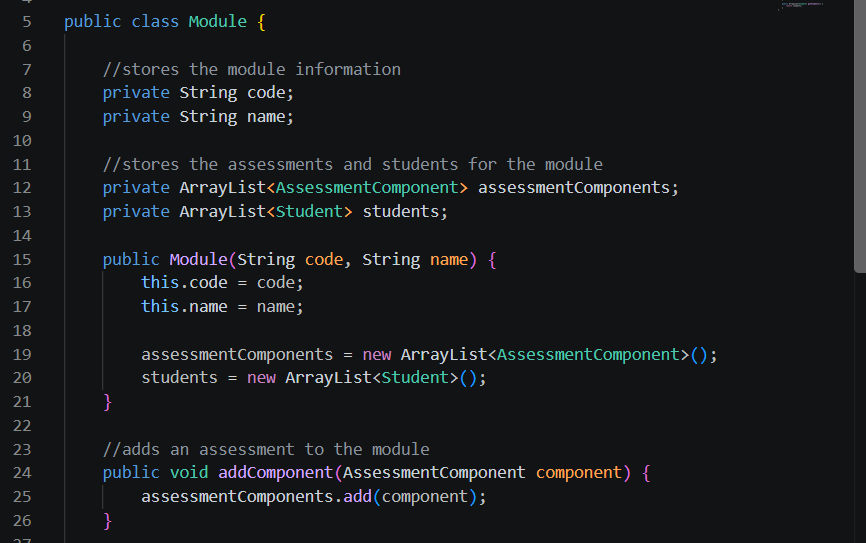
\includegraphics[width=0.95\textwidth]{Images/ch4_module_class.png}
    \caption{Module class attributes, constructor and assessment-component method.}
    \label{fig:ch4-module-class}
\end{figure}

\subsection{AssessmentComponent Class}

The \texttt{AssessmentComponent} class represents an individual assessment within a module. It stores the information required to identify an assessment and define its contribution to the module's assessment structure. Each object represents one assessment component, such as a test, practical or examination.

This class has four variables. A \texttt{key} variable is used to identify the assessment. The \texttt{label} variable stores the name of the assessment. A \texttt{weight} variable determines how much the assessment counts towards the total module result. A \texttt{maxMark} variable is used to store the maximum mark attainable for the assessment. This allows the assessment components to be described individually and provides the necessary information for the marking functionality.

All four variables are assigned values by the constructor. This means that the key details of the assessment and the calculation details are passed in when creating an \texttt{AssessmentComponent} object. There are four accessor methods included in the class: \texttt{getKey()}, \texttt{getLabel()}, \texttt{getWeight()} and \texttt{getMaxMark()}. This allows other classes to access the details of the assessment without compromising the private variables.

Private attributes are used to support encapsulation by limiting direct access to an object's internal data \cite{geeksEncapsulation}. The accessor methods allow other components to get the information that they need. For example, the \texttt{IndividualMarksManager} class uses the weighting and maximum mark attributes from the assessment components to work out the weighted contribution to an individual's result.

\begin{figure}[htbp]
    \centering
    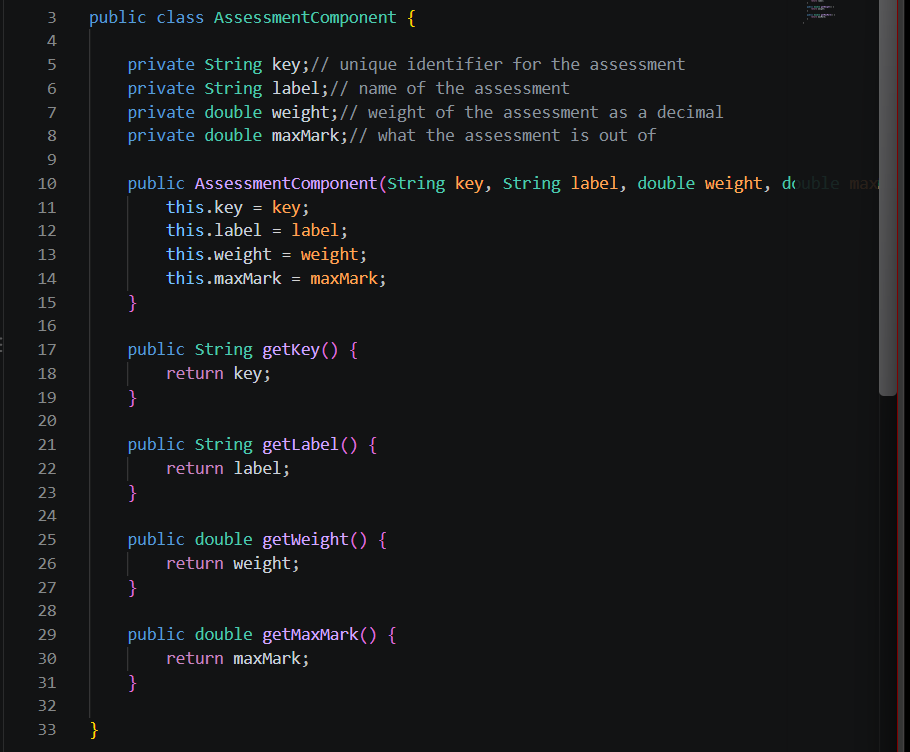
\includegraphics[width=0.95\textwidth]{Images/ch4_assessment_component.png}
    \caption{AssessmentComponent attributes, constructor and calculation-related accessor methods.}
    \label{fig:ch4-assessment-component}
\end{figure}

\subsection{IndividualMarksManager Class}

This class is responsible for managing an individual's marks within the three different assessment types: test, practical and examination. It contains the functionality to record marks, ensure they are valid, find out if any assessments have been missed and calculate performance statistics. This differs from the \texttt{Module} and \texttt{AssessmentComponent} classes because it contains the processing functionality.

There are three \texttt{Double} attributes: \texttt{testMark}, \texttt{practicalMark} and \texttt{examMark}. They are used to store the marks attained in each category of assessment. The attributes are declared as \texttt{Double} wrapper objects rather than primitive \texttt{double} values so that they can contain \texttt{null} values \cite{oracleDouble}. This is useful because the program can distinguish between a mark that has not yet been entered and a mark of zero. There are also three \texttt{AssessmentComponent} objects referenced by the class: \texttt{test}, \texttt{practical} and \texttt{exam}. These allow access to the maximum mark and weighting for each assessment.

\begin{figure}[htbp]
    \centering
    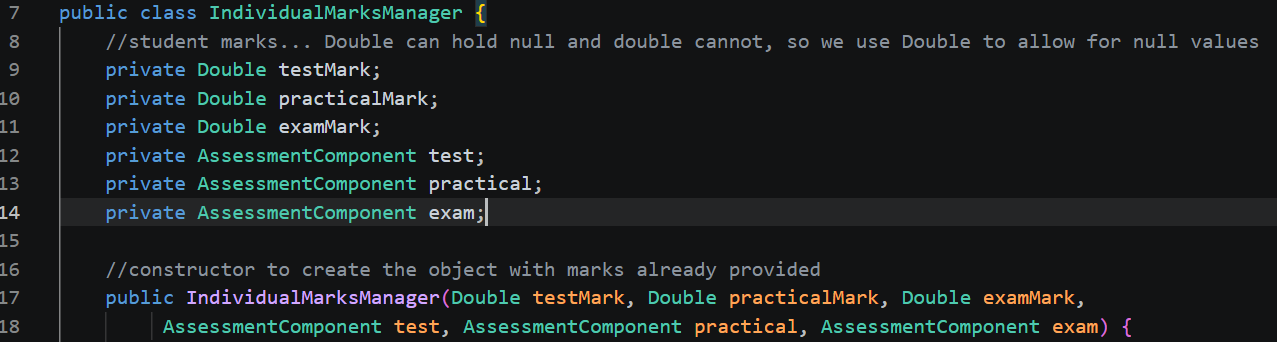
\includegraphics[width=0.95\textwidth]{Images/ch4_individual_marks_manager.png}
    \caption{IndividualMarksManager attributes and constructor structure.}
    \label{fig:ch4-individual-marks-manager}
\end{figure}

The constructor takes three marks and the corresponding assessment criteria. Before adding the marks, it ensures that any non-null marks are within the valid range of 0--100. If they are not, an \texttt{IllegalArgumentException} is thrown to prevent them from being added. This validation is also performed when marks are updated using the \texttt{setTestMark()}, \texttt{setPracticalMark()} and \texttt{setExamMark()} methods. This is done using a private method called \texttt{isValidMark()}.

\begin{figure}[htbp]
    \centering
    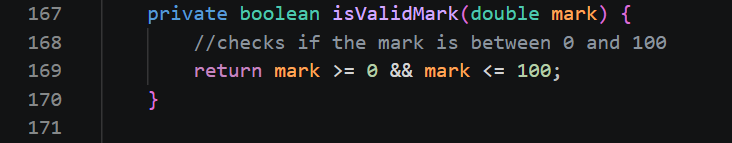
\includegraphics[width=0.82\textwidth]{Images/ch4_validation.png}
    \caption{Validation method enforcing the permitted mark range.}
    \label{fig:ch4-validation}
\end{figure}

This class also has methods to allow incomplete assessment data. The \texttt{hasMissingMarks()} method checks whether any of the three mark variables are \texttt{null}. If the data is incomplete, the \texttt{getMissingMarks()} method identifies which assessment category the mark is missing for. The methods for calculating results use this to stop calculations being performed when assessment data is incomplete. An \texttt{IllegalStateException} is thrown if a result calculation is attempted while marks are missing.

\begin{figure}[htbp]
    \centering
    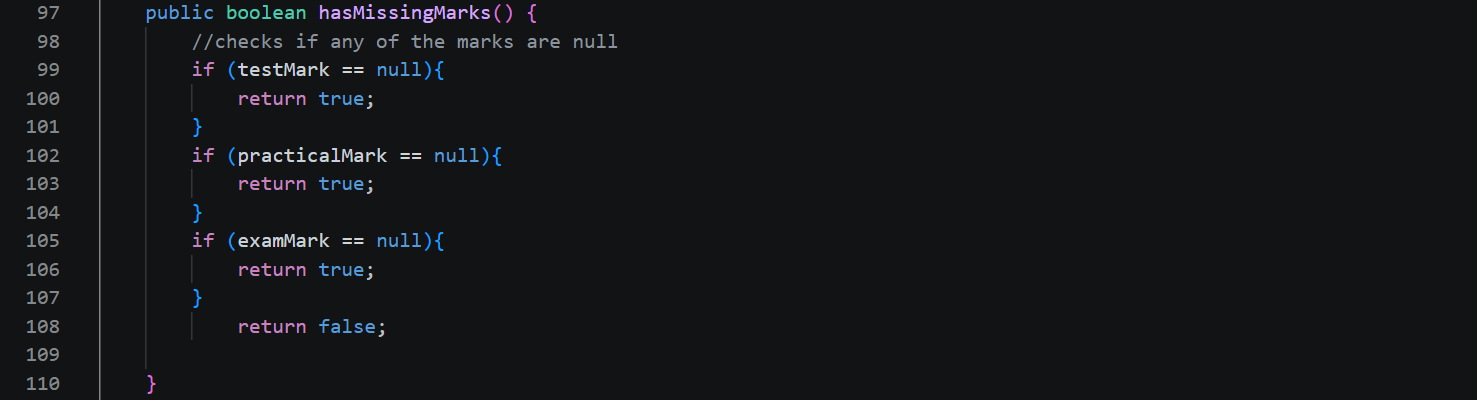
\includegraphics[width=0.95\textwidth]{Images/ch4_missing_marks_code.png}
    \caption{Detection of incomplete individual assessment records.}
    \label{fig:ch4-missing-marks-code}
\end{figure}

The class has various functions that can be used once the assessment records are complete. These include calculating the weighted final mark, average mark, highest mark and lowest mark. The weighted final mark is calculated by using the maximum mark and weighting of each \texttt{AssessmentComponent} in the \texttt{calculateFinalMark()} method. The average mark is the arithmetic mean of the three marks stored in the \texttt{calculateAverage()} method. The highest and lowest marks are found using the \texttt{getHighestMark()} and \texttt{getLowestMark()} methods.

\begin{figure}[htbp]
    \centering
    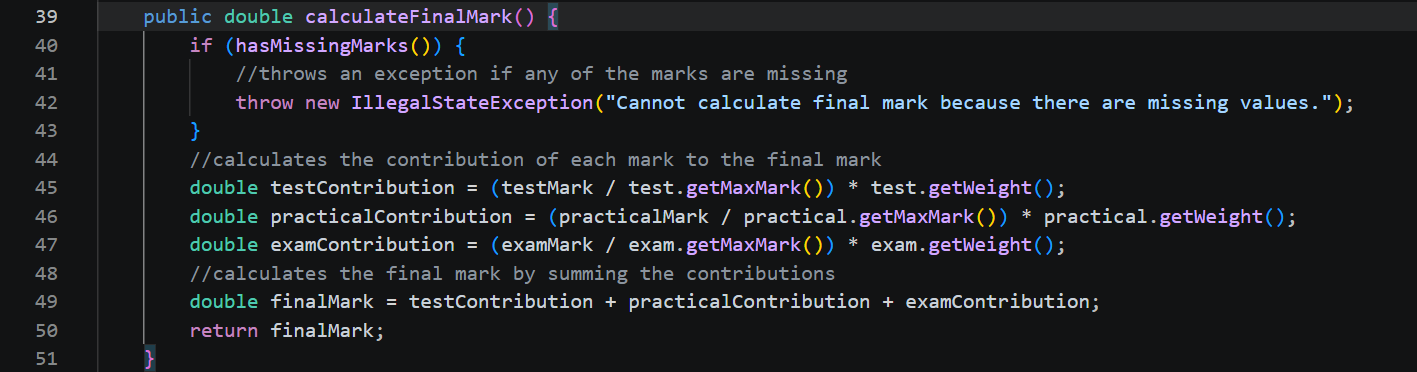
\includegraphics[width=0.95\textwidth]{Images/ch4_weighted_calculation.png}
    \caption{Calculation of the weighted contributions from the three assessment components.}
    \label{fig:ch4-weighted-calculation}
\end{figure}

This class allows marks to be stored, checked and calculated in one place. The ability to have nullable marks means that incomplete data can be identified, while validation and exception handling prevent calculations from being performed with incorrect or incomplete data.

\section{Class Relationships and Integration}

The \texttt{Module}, \texttt{AssessmentComponent} and \texttt{IndividualMarksManager} classes provide a means to manage individual assessment data. The classes have been designed so that each performs its own role to provide an effective way to handle module details, assessments and individual marks.

The \texttt{Module} class has an attribute called \texttt{assessmentComponents}, which contains a collection of \texttt{AssessmentComponent} objects. This is an example of a one-to-many relationship between the two classes. A module can have many assessment components, each representing a different form of assessment within that module. This provides a way of storing assessment-related information in relation to the module.

The \texttt{IndividualMarksManager} contains three references (\texttt{test}, \texttt{practical} and \texttt{exam}) to \texttt{AssessmentComponent} objects. These references provide access to the maximum mark and weightings required to calculate how much each assessment component contributes to the individual's final result. Each of the marks for the assessments is stored in the \texttt{testMark}, \texttt{practicalMark} and \texttt{examMark} attributes.

\begin{figure}[htbp]
    \centering
    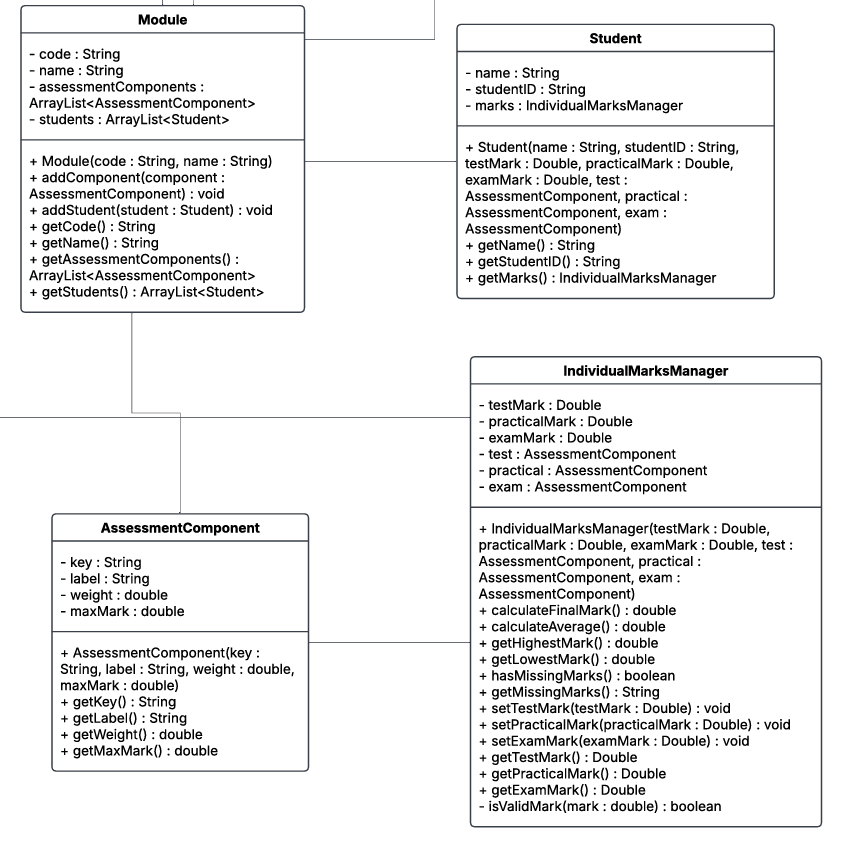
\includegraphics[width=0.9\textwidth]{Images/ch4_marks_uml.png}
    \caption{Relationships between the marks-management classes.}
    \label{fig:ch4-marks-relationships}
\end{figure}

This creates a flow of data between these classes where the \texttt{Module} class manages the assessment components, the \texttt{AssessmentComponent} class determines the assessment parameters and the \texttt{IndividualMarksManager} uses these to process individual marks. This allows the code to have a modular design, making it easier to identify the responsibility of each class.

\section{Testing Methodology}

The three classes were tested both individually and by integrating them into a demonstration application. This application included creating a module, adding the assessment components, recording individual marks and calculating their performance.

Additional scenarios were used to test the functionality of incomplete assessment records and mark updates. Results from the console were checked to make sure they were correct.

\section{Testing Results and Evidence}

The practical tests showed that the three classes were working as expected. The system was able to display the module and its assessments, enter individual marks and calculate performance statistics. The missing-record test showed that when a mark was missing, it was identified and calculations were prevented until the mark had been entered. When the practical mark was updated, the system correctly recalculated the student's results. All tests ran successfully once the missing record was dealt with.

\begin{table}[htbp]
    \centering
    \caption{Testing scenarios and observed results.}
    \label{tab:ch4-testing}
    \begin{tabular}{|p{0.42\textwidth}|p{0.48\textwidth}|}
        \hline
        \textbf{Test scenario} & \textbf{Observed result} \\
        \hline
        Complete marks record & Performance statistics calculated successfully \\
        \hline
        Missing assessment mark & Missing mark identified and calculations prevented \\
        \hline
        Updated assessment mark & Record updated and results recalculated \\
        \hline
    \end{tabular}
\end{table}

Console screenshots are included as evidence of the practical test scenarios and their corresponding outputs.

\begin{figure}[htbp]
    \centering
    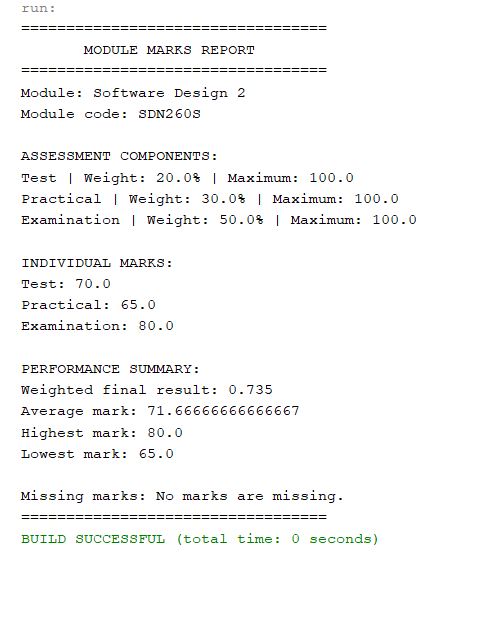
\includegraphics[width=0.72\textwidth]{Images/ch4_complete_marks_test.png}
    \caption{Successful processing of a complete individual marks record.}
    \label{fig:ch4-complete-marks-test}
\end{figure}

\begin{figure}[htbp]
    \centering
    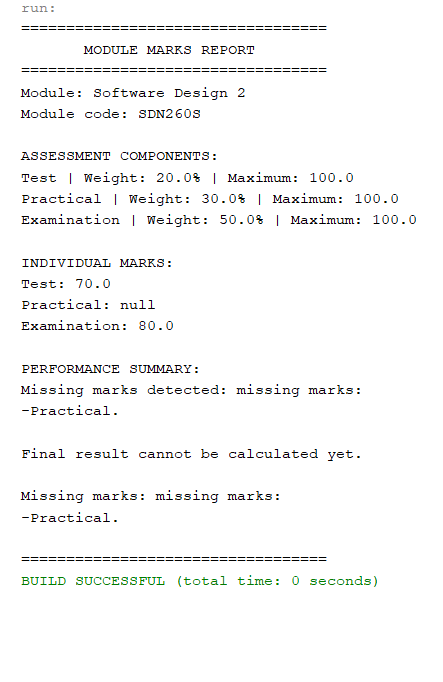
\includegraphics[width=0.72\textwidth]{Images/ch4_missing_mark_test.png}
    \caption{Detection of a missing assessment mark.}
    \label{fig:ch4-missing-mark-test}
\end{figure}

\begin{figure}[htbp]
    \centering
    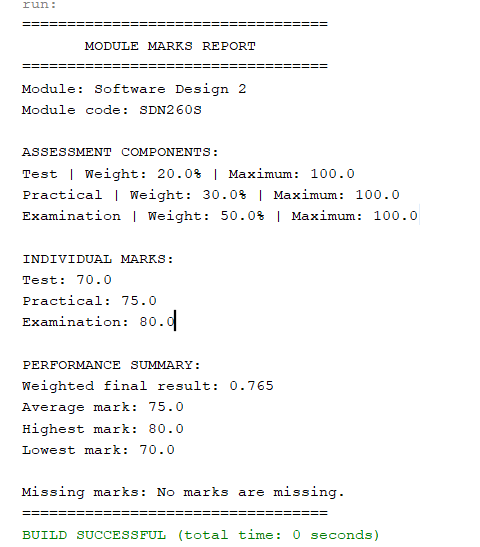
\includegraphics[width=0.72\textwidth]{Images/ch4_updated_mark_test.png}
    \caption{Updated individual marks record and recalculated performance results.}
    \label{fig:ch4-updated-mark-test}
\end{figure}

\section{Troubleshooting and Identified Issues}

During the implementation and testing of the demonstration program, an issue occurred when trying to calculate results from an incomplete marks record. Although the \texttt{IndividualMarksManager} correctly threw an \texttt{IllegalStateException} because marks were incomplete, the demonstration program initially did not handle this before attempting the calculation and therefore terminated.

This was solved by first checking whether any marks were missing. The program identifies which assessment marks are missing and prevents calculations from taking place until the missing marks have been entered.

Another test was conducted to show that when the missing practical mark was updated, the system correctly recalculated the student's results. This shows the importance of managing incomplete assessment data.

\section{Conclusion}

This chapter has discussed the design, implementation and testing of the \texttt{Module}, \texttt{AssessmentComponent} and \texttt{IndividualMarksManager} classes. These classes support the organisation of module assessment components, the storage of assessment information and the management of individual student marks.

The classes have been tested practically and shown to work together to process complete mark records, identify missing marks for assessments and recalculate results when marks have been updated. This provides the fundamental functionality needed to manage individual assessment information.

\section{Authorship and Originality Statement}

This chapter has been constructed based on the marks-management components that I implemented, tested and understood as part of the group project. Code examples, testing results and screenshots have been included to provide evidence of my implementation. Writing tools were used to assist with the organisation and formatting of the technical information. The observations, implementation details and results presented in this chapter are based on the work completed for my assigned section of the project.
